    \documentclass[11pt]{article}
    %	options include 12pt or 11pt or 10pt
    %	classes include article, report, book, letter, thesis
    
    \title{HW4}
    \author{Shane Drafahl}
    \date{16 October ,2017}
    \usepackage{graphicx}
    \usepackage{epstopdf}
    \usepackage{graphics}

    \begin{document}
    \maketitle

    1. $ \newline \newline $

    \begin{figure}[!htb]
        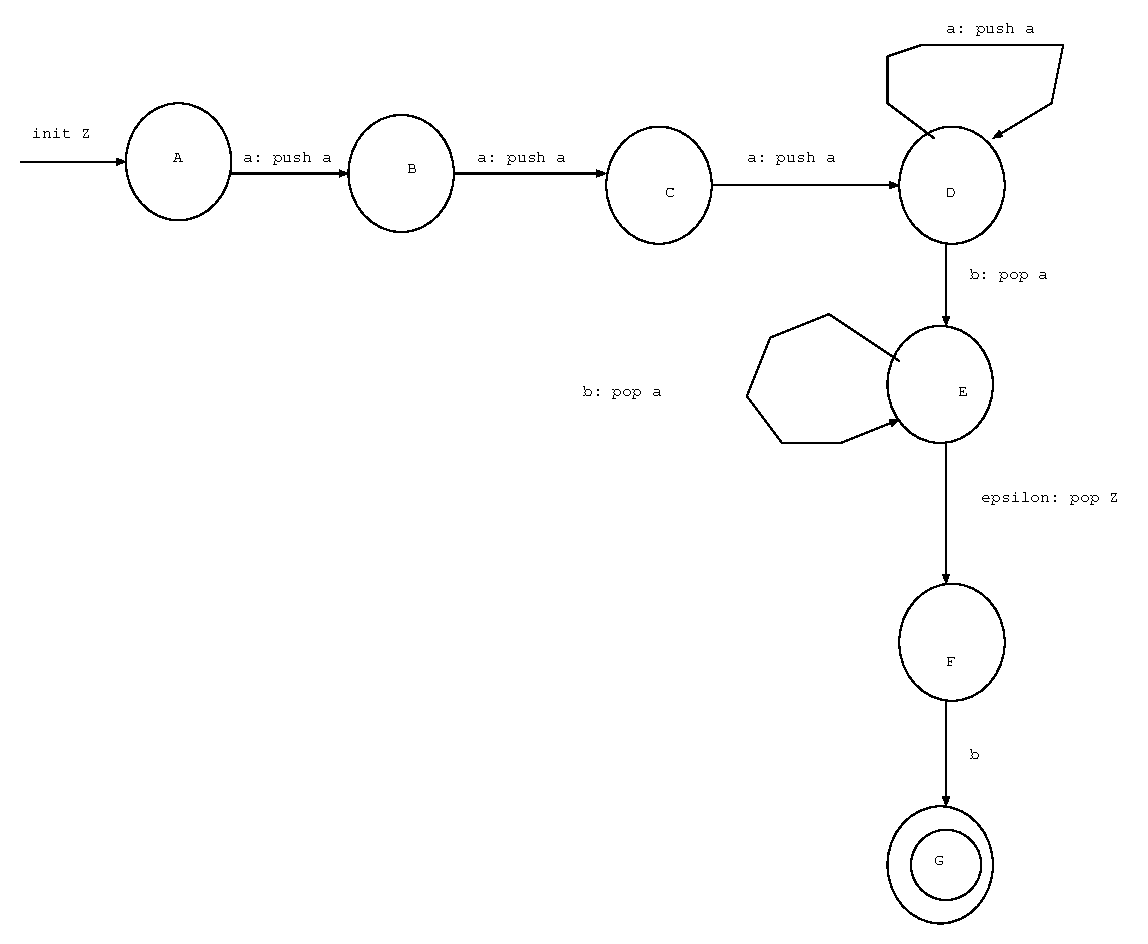
\includegraphics[scale=.6]{./hw8_1.eps}
    \end{figure}

    $ \newline $

    2.

    $ \newline $

    By contradiction if we assume that this language is context-free. So
    there would be an m such that any string $ w \in L $, $ |w| \geq m $. 
    We will choose w = $ b^{m}a^{m+1}b^{m} $. w cannot be decomposed into w = $ uv^{k}xy^{k}z $ where 
    k is a natural number.
    $ \newline $
    case 1: vxy are composed of all a's. If k = 0 then there will be at least one less a meaning that at least the
    longest run of a's and b's would be equal or the longest run of b's would be longer.
    $ \newline $
    case 2: vxy are composed of all b's. If k = 1 then at least there would be one additional b. Meaning  that at least the 
    longest run of a's and b's would equal otherwise the longest run of b's would be longer.
    $ \newline $
    case 3: vxy are compose of a's and b's. vxy cannot be greater than m so either the middle and left 
    run or the middle and right run can be pumped at most. Also because of the restriction 
    that v and y cannot be both epsilon we know that we will either pump just b's , just a's or both a's and b's.
    If we pump just a's or just b's k = 1 for just b's and k = 0 for just a's similar to case 1 and 2. Otherwise if 
    we pump both a's and b's if k = 0 then there will be one less a or b in either of the runs. This will mean one of the 
    runs of b's will now be equal or longer than the runs of a's.

    $ \newline $

    3. Using proof by contradiction we will assume that the given language is context free. Therefore it can be pumped
    using pumping lemma. First we will pick a string in the language $ z \in L $. $ z = 1^{m}0^{m+1}21^{m+1}0^{m} $ where 
    $ z \geq m $ and that z is divided up between uvxyz where $ m \leq | v^{k}xy^{k} |$. There are three cases to this problem.

    $ \newline $

    Case 1: If the left side of the 2 is only pumped and k is greater than 1. In this case because both sides are equal in length the alpha value 
    will be greater than the beta so it cannot be in the string.

    $ \newline $

    Case 2: If the right side of the 2's is pumped then if we underpumped it a similar senario to case would happen. If we underpump it
    then alpha will have more bits and will be greater in value.

    $ \newline $

    Case 3: If the uvx split up between both sides of the 2. In this case if v or the y are not equal in the number of bits
    to each other then this is similar to case 1 and 2. If more bits from alpha are in v then there are bits from beta in y then 
    you pump it making alpha a larger value. This is symetric if y has a larger cardinality than v. Otherwise if $ |v| = |y| $ then 
    if we underpump v and y the string goes from $ 1^{m}0^{m+1}21^{m+1}0^{m} $ to $ 1^{m}0^{m}21^{m}0^{m} $. The resulting string 
    after pumping the alpha will either be equal to or greater than the beta. Therefore by proof of contradiction L is not context free.
    

    $ \newline $
    This answer was enspired by 
    $ \newline $
    https://cs.stackexchange.com/questions/82637/prove-or-disprove-that-the-following-language-is-context-free

    
    \end{document}